\section{Experiments}

% \input{tables/simulation}

\subsection{Settings}
\label{sec: setting}
\paragraph{Models.} We evaluate \kivi{} using three popular model families: Llama/Llama-2~\citep{touvron2023llama, touvron2023llama2}, Falcon~\citep{penedo2023refinedweb} and Mistral~\citep{jiang2023mistral}. 
Llama and Mistral model is based on multi-head attention, while Falcon is based on multi-query attention \citep{mqa}.
We use the Hugging Face Transformers codebase and implement the \kivi{} algorithm upon it.
Following previous work \citep{flexgen}, the group size $G$ in Algorithm \ref{algo: kivi} for quantization is set as 32 across all experiments, the residual length $R$ for key and value cache is set to 128.

\paragraph{Tasks.}
As we analyzed in Section \ref{sec: background}, the KV cache size grows larger with a longer context. 
Thus, we evaluate \kivi{} under the normal context length and long context setting, respectively.
Specifically, we adopt generation tasks from LM-Eval~\citep{eval-harness} for normal context length evaluation and LongBench~\citep{bai2023longbench} for long context evaluation, respectively\footnote{The closed-end tasks such as MMLU are not ideal to evaluate \kivi{} since they only involve one decoding step and directly fetch the output logits, which is not suitable for studying the impact of compressed KV cache.}. 
For LM-eval, we adopt CoQA (Exact match accuracy), TruthfulQA (BLEU score), and GSM8K (Exact match accuracy). 
For LongBench, we chose tasks from four subgroups. 
Specifically, Qasper (F1 score) is a Single-Document QA task; QMSum (ROUGE score) and MultiNews (ROUGE score) are Summarization tasks; TREC (classification score), TriviaQA (F1 score), and SAMSum (ROUGE score) are Few-shot Learning tasks; and LCC (similarity score) and RepoBench-P (similarity score) is Code Completion task. The maximum sequence length in LongBench was set to 8192 for the Mistral model and 4096 for other models.
We also consider the needle-in-a-haystack task (NIAH) to evaluate the model's long context retrieval ability after quantizing KV cache.
Detailed NIAH setting can be found in Appendix \ref{app: niah}.

\subsection{Accuracy and Efficiency Analysis}

\subsubsection{Comparison Between Different Quantization Configurations}

We first utilize the fake quantization to demonstrate the effectiveness of our asymmetric quantization, namely, quantizing key cache per-channel and value cache per-token. 
Here fake quantization is exactly the same as in Table \ref{tab:sub_simulation}.
The results are shown in Table \ref{tab:merged-lm-eval}.
We observe that ``2bit (K per-channel, V per-token)'' consistently achieves the best results compared to all other configurations.
This is consistent with our previous analysis.
We also note that for hard generation tasks such as GSM8K, the fake ``2bit (K per-channel, V per-token)'' quantization results are significantly worse than the full precision counterparts.
However, for \kivi{} in Table \ref{tab:merged-lm-eval}, we observe that the accuracy drop is only around $2\%$ for GSM8K across different models.
As we analyzed in Section \ref{sec: algo},
the difference between fake ``2bit (K per-channel, V per-token)'' quantization and \kivi{} is that \kivi{} maintains a full precision key and value cache sliding window for the local relevant tokens.
This sliding window is crucial to maintaining accuracy for hard generation tasks such as mathematical reasoning. 

\subsubsection{Accuracy Comparison on Generation Tasks}

% \begin{table}
% \centering
% \caption{Performance comparison between 16bit, four fake 2bit KV cache quantization similar to those in Table \ref{tab:sub_simulation}, \kivi-2 (2bit)/\kivi-4 (4bit) across various models.
% We emphasize that unlike \kivi which preserve a small portion of full precision key cache $\mX_{K_r}$, all tokens in fake KV cache quantization are quantized for a fair comparison.
% Falcon adopts multi-query attention and only has one head for KV cache.
% Thus it is already highly compressed and 4-bit \kivi may needed to maintain the accuracy in this case.}
% \label{tab:merged-lm-eval}
% \begin{tabular}{llccc} 
% \hline
% \multicolumn{2}{l}{\textbf{Model}}        & \textbf{CoQA} & \textbf{TruthfulQA} & \textbf{GSM8K}  \\
% \hline
% % \multirow{2}{*}{Llama-7B}    & 16bit  &      62.67      &          25.78    &   9.10       \\
% %             & kivi-2 &      62.60     &        23.51    &    7.05        \\
% % \hline
% % \multirow{2}{*}{Llama-13B}   & 16bit  &      63.80     &          26.35     &   17.06       \\
% %             & kivi-2 &      63.18       &         25.14     &    14.86     \\
% % \hline
% \multirow{6}{*}{Llama-2-7B}  & 16bit  &     63.88      &         30.76        &   13.50     \\
% \cline{2-5}
%  & 2bit (K per-channel, V per-token)  & 61.18 & \bf{33.39} & 2.35 \\
%  & 2bit (K per-token, V per-token)     & 60.57 & 28.22 & 0.68 \\
%  & 2bit (K per-channel, V per-channel) & 36.23 & 0.13 & 0.00\\
%  & 2bit (K per-token, V per-channel)   & 37.72 & 0.14 &  0.00 \\
%             & kivi-2 &      \bf{61.80}     &          32.80        &    \bf{11.22}   \\
% \hline
% \multirow{6}{*}{Llama-2-13B} & 16bit  &      66.37     &        29.53        &   22.67      \\
% \cline{2-5}
%  & 2bit (K per-channel, V per-token)  & 65.70 & 29.32  & 3.49 \\
%  & 2bit (K per-token, V per-token)   & 63.10 & 24.81 & 1.67  \\
%  & 2bit (K per-channel, V per-channel) & 38.45 & 1.89 & 0.08  \\
%  & 2bit (K per-token, V per-channel)   & 33.45 & 2.27 &  0.08 \\
%             & kivi-2 &    \bf{65.93}    &        \bf{29.51}          &     \bf{18.88}     \\
% \hline
% \multirow{7}{*}{Falcon-7B}   & 16bit  &     59.83   &   23.20    &        4.55          \\
% \cline{2-5}
%  & 2bit (K per-channel, V per-token)   & 54.13 & 21.73 & 0.76  \\
%  & 2bit (K per-token, V per-token)    & 45.30 & 7.98 &  0.38 \\
%  & 2bit (K per-channel, V per-channel) & 51.38 & 14.97 & 0.53  \\
%  & 2bit (K per-token, V per-channel)   & 41.22 & 1.41 & 0.15 \\
%             & kivi-4 &     \bf{60.17}      &   22.94    &       \bf{3.49}           \\
%             & kivi-2 &     53.90      &  \bf{23.46}     &       1.97        \\
% \hline
% \end{tabular}
% \end{table}



\begin{table}[h!]
\centering
\caption{Performance comparison between 16bit, 4-bit per-token quantization, four fake 2bit KV cache quantization similar to those in Table \ref{tab:sub_simulation}, \kivitwo{} (2bit) / \kivifour{} (4bit) across various models.
We emphasize that unlike \kivi{}, which preserves a small portion of full precision key cache $\mX_{K_r}$ and value cache $\mX_{V_r}$, all tokens in fake KV cache quantization are quantized for a fair comparison.
$\mathbb{C}$ stands for per-channel quantization and $\mathbb{T}$ stands for per-token quantization.}
\label{tab:merged-lm-eval}
\resizebox{\linewidth}{!}{
\begin{tabular}{llccc} 
\toprule
\multicolumn{2}{l}{\textbf{Model}}        & \textbf{CoQA} & \textbf{TruthfulQA} & \textbf{GSM8K}  \\
\midrule
\multirow{8}{*}{Llama-2-7B}  & 16bit  &     63.88      &         30.76        &   13.50     \\
 & 4bit (K - $\mathbb{T}$, V - $\mathbb{T}$) & 64.82 & 29.85 & 12.28 \\
\cmidrule{2-5}
 & 2bit (K - $\mathbb{C}$, V - $\mathbb{T}$)  &  59.08 & 33.10 & 5.76 \\
 & 2bit (K - $\mathbb{T}$, V - $\mathbb{T}$)     &  39.88 & 18.29 & 0.83 \\
 & 2bit (K - $\mathbb{C}$, V - $\mathbb{C}$) & 3.60 & 0.27 & 0.00 \\
 & 2bit (K - $\mathbb{T}$, V - $\mathbb{C}$)   & 1.30 & 0.49 & 0.08\\
 % & kivi-2 (w/o buffer) & 61.80 & 32.80 & 11.22 \\
 & \kivifour{} & 63.78 & 30.80 & 13.80 \\
 & \kivitwo{} &  63.05 & 33.95 & 12.74 \\
\midrule
\multirow{8}{*}{Llama-2-13B} & 16bit  &      66.37     &        29.53        &   22.67      \\
 & 4bit (K - $\mathbb{T}$, V - $\mathbb{T}$)  & 66.73 & 29.14 & 20.92 \\
\cmidrule{2-5}
 & 2bit (K - $\mathbb{C}$, V - $\mathbb{T}$)  & 63.53 & 28.60 & 12.21 \\
 & 2bit (K - $\mathbb{T}$, V - $\mathbb{T}$)   & 52.93 & 24.98 & 4.55 \\
 & 2bit (K - $\mathbb{C}$, V - $\mathbb{C}$) & 2.88 & 0.74 & 0.00 \\
 & 2bit (K - $\mathbb{T}$, V - $\mathbb{C}$)   & 2.80 & 0.26 & 0.08 \\
 % & kivi-2 (w/o buffer) & 65.93 & 29.51   &  18.88 \\
 & \kivifour{} & 66.38 & 29.49 & 23.65\\
 & \kivitwo{} & 66.23 & 29.84  & 20.77 \\
\midrule
\multirow{8}{*}{Falcon-7B}   & 16bit  &     59.83   &   23.20    &        4.55          \\
 & 4bit (K - $\mathbb{T}$, V - $\mathbb{T}$)  & 58.53 & 22.94 & 3.26\\
\cmidrule{2-5}
 & 2bit (K - $\mathbb{C}$, V - $\mathbb{T}$)   &  43.93 & 20.82 & 1.29 \\
 & 2bit (K - $\mathbb{T}$, V - $\mathbb{T}$)    & 25.72 & 0.91 & 0.53 \\
 & 2bit (K - $\mathbb{C}$, V - $\mathbb{C}$) & 41.95 & 17.11 & 1.52 \\
 & 2bit (K - $\mathbb{T}$, V - $\mathbb{C}$)   & 19.53 & 0.94 & 0.15 \\
 & \kivifour{} & 59.67 & 22.58 & 4.47 \\
 & \kivitwo{} & 57.48 & 24.98 & 3.41 \\
\midrule
\multirow{8}{*}{Mistral-7B}   & 16bit  &     67.40  &  30.45  &  38.36     \\
 & 4bit (K - $\mathbb{T}$, V - $\mathbb{T}$)  & 67.80 & 29.83 & 36.85 \\
\cmidrule{2-5}
 & 2bit (K - $\mathbb{C}$, V - $\mathbb{T}$)   & 61.65 & 29.64 & 26.46 \\
 & 2bit (K - $\mathbb{T}$, V - $\mathbb{T}$)     & 54.55 & 25.86 & 5.00 \\
 & 2bit (K - $\mathbb{C}$, V - $\mathbb{C}$) & 24.40 & 24.86 & 2.27  \\
 & 2bit (K - $\mathbb{T}$, V - $\mathbb{C}$)   & 10.73 & 19.12 & 0.99 \\
 % & kivi-2 (w/o buffer) & 66.45 & 29.76 & 28.73 \\
 & \kivifour{} & 66.95 & 30.49 & 37.30\\
 & \kivitwo{} & 66.35 & 32.17 & 36.01  \\
\bottomrule
\vspace{-1.5em}
\end{tabular}
}
\end{table}

\begin{table*}[t]
\centering
\caption{Performance evaluation of \kivi{} on various models across a range of benchmarks in LongBench. We highlight the average performance of our method.
\textbf{More similar results on Mistral-7B-v0.2 and LongChat-7b-v1.5 can be found in Table \ref{table:longchat} and Table \ref{table:mistral}}}
\label{tab:longbench}
\resizebox{\textwidth}{!}{
\begin{tabular}{llccccccccc} 
\toprule
\multicolumn{2}{l}{\textbf{Model}}    & \textbf{Qasper} & \textbf{QMSum} & \textbf{MultiNews} & \textbf{TREC} & \textbf{TriviaQA} & \textbf{SAMSum} & \textbf{LCC} & \textbf{RepoBench-P} & \textbf{Average}  \\ 
\midrule
\multirow{3}{*}{Llama2-7B}      & 16bit  & 9.52 & 21.28 & 3.51 & 66.00 & 87.72 & 41.69 & 66.66 & 59.82 & 44.52  \\
                                & \kivifour{} & 9.28 & 21.42 & 3.88 & 66.00 & 87.72 & 41.82 & 66.80 & 59.83 & 44.59\\
                                & \kivitwo{} & 9.31 & 20.50 & 1.14 & 66.00 & 87.42 & 42.71 & 66.88 & 60.23 & \textbf{44.27} \\
\midrule
\multirow{3}{*}{Llama2-13B}     & 16bit  & 9.32 & 21.38 & 3.71 & 70.00 & 87.87 & 43.55 & 66.61 &56.42 & 44.85 \\
                                & \kivifour{} & 9.16 & 20.86 & 3.21 & 69.00 & 86.97 & 44.26 & 65.30 & 57.08 & 44.48\\
                                & \kivitwo{} & 8.58 & 20.69 & 6.19 & 69.50 & 87.78 & 44.30 & 65.08 & 55.46 & \textbf{44.69} \\
\midrule
\multirow{3}{*}{Llama2-7B-Chat} & 16bit  & 19.65 & 20.54 & 26.36 & 63.00 & 84.28 & 41.12 & 59.75 & 52.93 & 45.95 \\
                                & \kivifour{} & 19.62 & 20.70 & 25.49 & 63.00 & 84.13 & 40.87 & 59.27 & 53.56 & 45.83\\
                                & \kivitwo{} & 19.32 & 20.46 & 25.48 & 63.00 & 84.84 & 40.60 & 58.71 & 52.97 & \textbf{45.67} \\
\midrule
\multirow{3}{*}{Llama2-13B-Chat} & 16bit  & 24.18 & 20.37 & 25.69 & 67.50 & 86.90 & 42.18 & 50.23 & 50.64 & 45.96 \\
                                & \kivifour{} & 23.00 & 20.36 & 26.06 & 67.50 & 87.20 & 42.04 & 52.55 & 52.77 & 46.44\\
                                 & \kivitwo{} & 23.59 & 20.76 & 25.25 & 67.5 & 87.17 & 41.56 & 49.93 & 48.45 & \textbf{45.52} \\
\midrule
\multirow{3}{*}{Falcon-7B}      & 16bit  & 1.48 & 2.35 & 11.09 & 13.00 & 5.84 & 2.44 & 23.86 & 9.69 & 8.71 \\
                                & \kivifour{} & 1.04 & 2.41 & 11.98 & 13.00 & 5.84 & 2.36 & 23.72 & 9.92 & \textbf{8.78} \\
                                & \kivitwo{} & 1.98 & 3.61 & 6.78 & 10.00 & 6.24 & 2.73 & 22.18 & 10.12 & \textbf{7.95} \\
\midrule
\multirow{3}{*}{Mistral-7B}     & 16bit  & 8.12 & 19.98 & 19.99 & 67.50 & 89.80 & 41.69 & 66.59 & 58.99 & 46.58 \\
                                & \kivifour{} & 7.89 & 20.06 & 20.58 & 67.50 & 89.80 & 41.56 & 66.45 & 58.62 & 46.56 \\
                                & \kivitwo{} & 6.92 & 19.71 & 17.92 & 66.50 & 89.63& 41.66 & 65.52 & 58.99 & \textbf{45.85} \\
\bottomrule
\end{tabular}
}
\end{table*}

\begin{figure*}[h]
% \vspace{-1em}
\setlength{\abovecaptionskip}{0mm}
\setlength{\belowcaptionskip}{0mm}
\centering
\subfigcapskip=-2mm

\begin{minipage}{0.95\linewidth}
    
\subfigure[\!Llama-3-8B-Instruct Baseline]{
\centering
    % \begin{minipage}[t]{0.3\linewidth}
        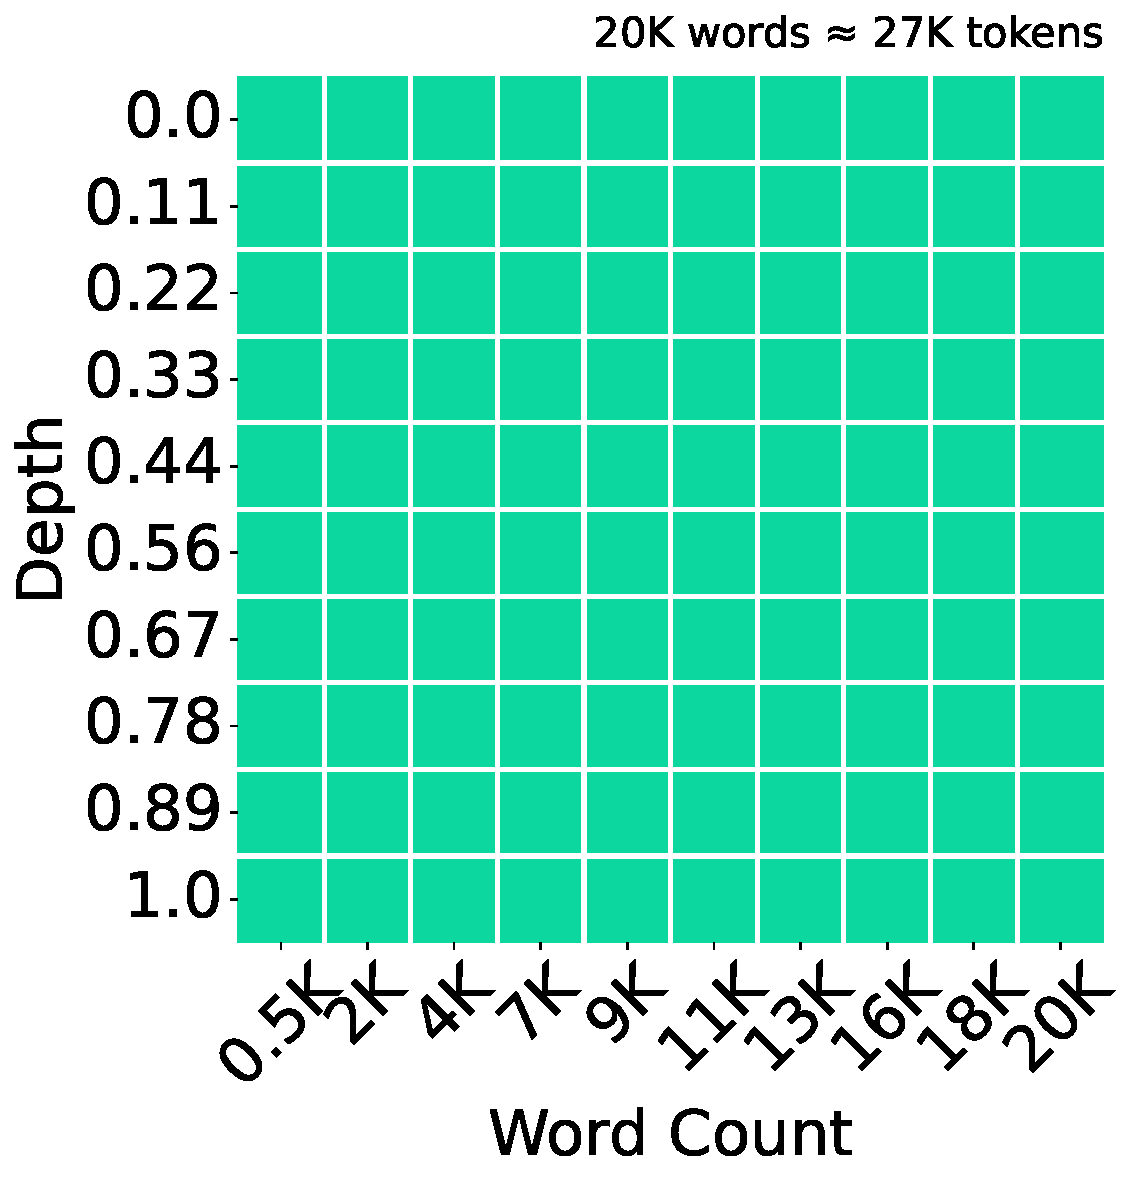
\includegraphics[width=0.3\linewidth]{figures/needle/icl_raw_extend/llama.pdf}
    % \end{minipage}%
}
\subfigure[\!Llama-3-8B-Instruct + \kivitwo{}]{
\centering
    % \begin{minipage}[t]{0.3\linewidth}
        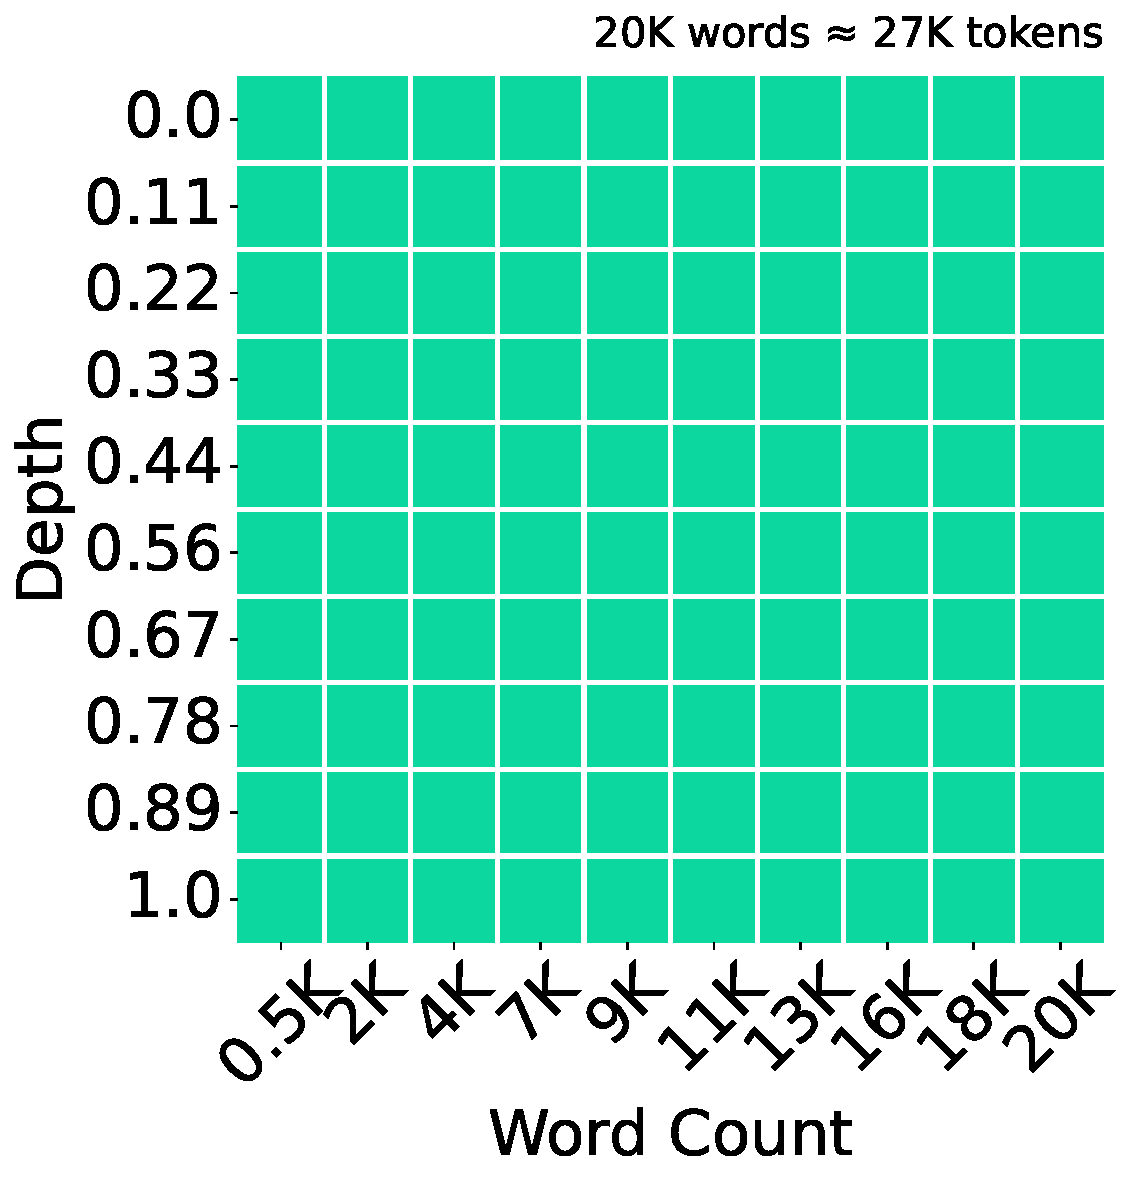
\includegraphics[width=0.3\linewidth]{figures/needle/kivi/llama/2_bit.pdf}
    % \end{minipage}%
}
\subfigure[\!Llama-3-8B-Instruct + \kivifour{}]{
\centering
    % \begin{minipage}[t]{0.3\linewidth}
        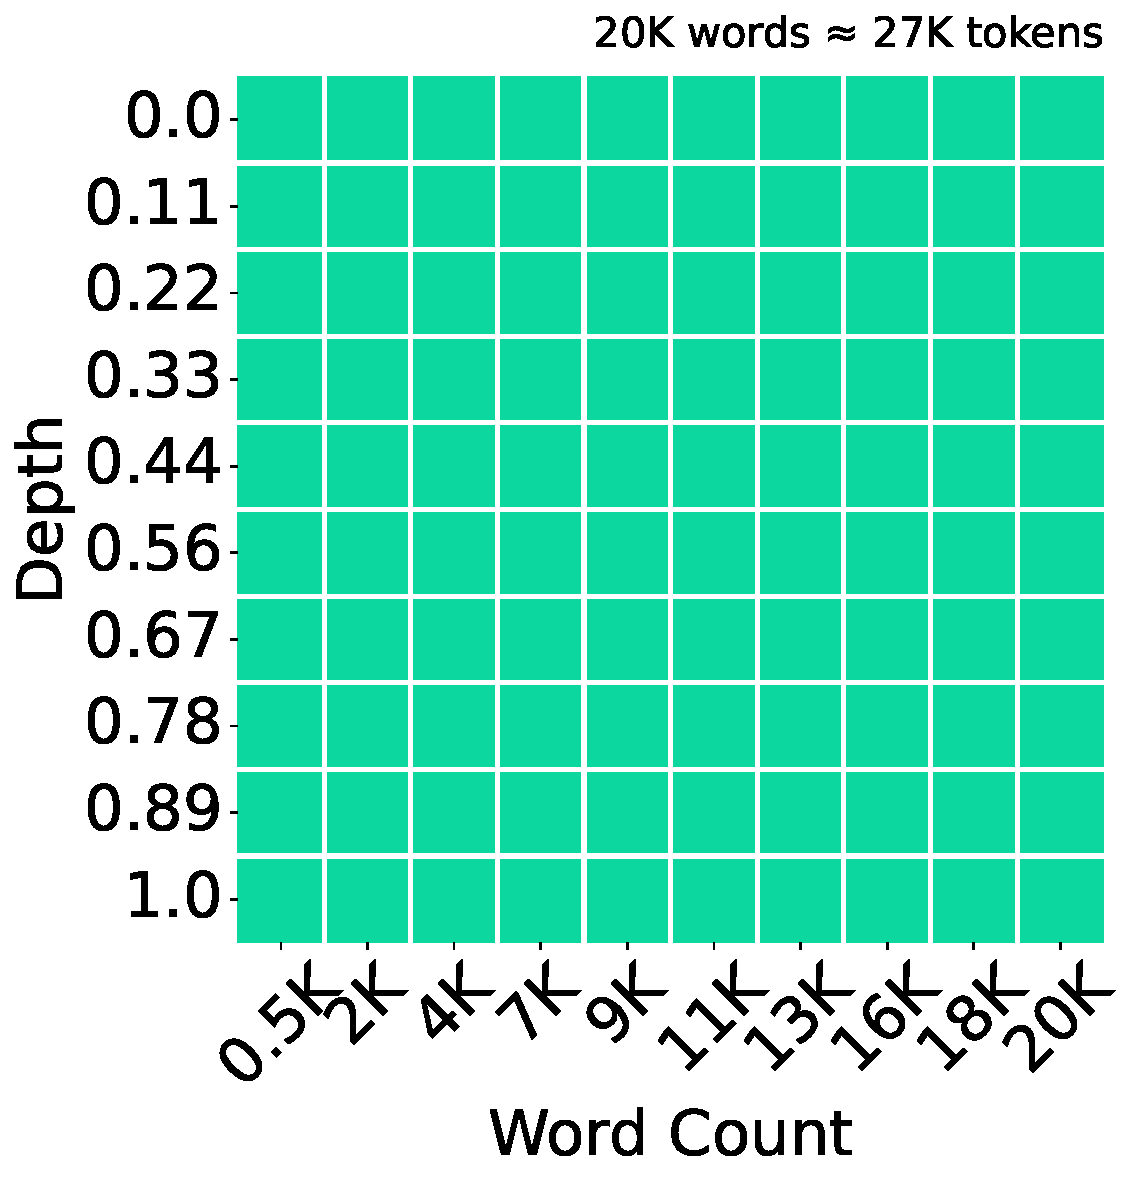
\includegraphics[width=0.3\linewidth]{figures/needle/kivi/llama/4_bit.pdf}
    % \end{minipage}%
}

\subfigure[\!Mistral-7B-Instruct-v0.2 Baseline]{
\centering
    % \begin{minipage}[t]{0.3\linewidth}
        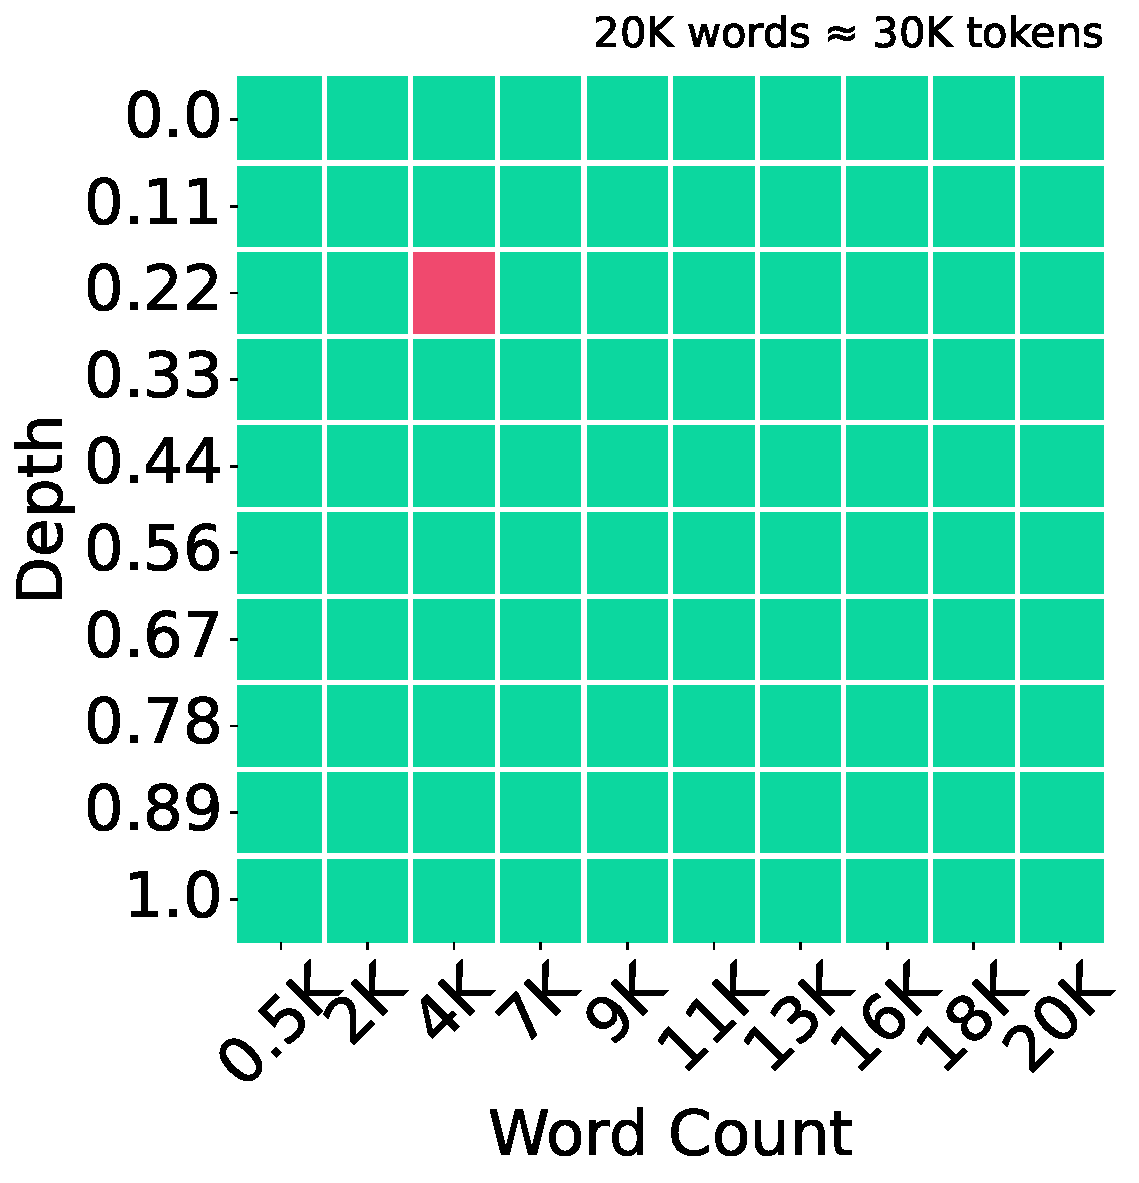
\includegraphics[width=0.3\linewidth]{figures/needle/icl_raw_extend/mistral.pdf}
    % \end{minipage}%
}
\subfigure[\!Mistral-7B-Instruct-v0.2 + \kivitwo{}]{
\centering
    % \begin{minipage}[t]{0.3\linewidth}
        
\includegraphics[width=0.3\linewidth]{figures/needle/kivi/mistral/2_bit.pdf}
    % \end{minipage}%
}
\subfigure[\!Mistral-7B-Instruct-v0.2 + \kivifour{}]{
\centering
    % \begin{minipage}[t]{0.3\linewidth}
        
\includegraphics[width=0.3\linewidth]{figures/needle/kivi/mistral/4_bit.pdf}
    % \end{minipage}%
}

\end{minipage}
\hspace{-1em}
\begin{minipage}{0.04\linewidth}
    \centering
    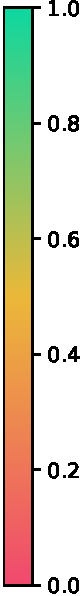
\includegraphics[width=1.25\linewidth]{figures/needle/bar2.pdf}
\end{minipage}

\caption{Needle-in-a-Haystack results on Llama-3-8B-Instruct and Mistral-7B-Instruct-v0.2. Here we count the number of words instead of tokens to better account for the tokenizer difference. The final token length is noted in the upper right corners of each figure. Detailed setting can be found in Appendix \ref{app: niah}.}
\label{fig: needle}
\end{figure*}

\paragraph{LM-Eval Results.}
We benchmark \kivi{} in CoQA, TruthfulQA and GSM8K tasks using the LM-Eval framework. All dataset parameters were set to default. We compare the standard 16bit configuration with our \kivi{} compression techniques in Llama-2-7B, Llama-2-13B, Falcon-7B and Mistral-7B. As shown in Table ~\ref{tab:merged-lm-eval}, we observe that for the Llama and Mistral model, \kivi{} only has up to 2\% accuracy drop despite the KV cache being stored in 2bit.
For instance, in the Llama-2-7B model, the transition from 16bit to 2bit only slightly decreases accuracy. 
Similar trends are observed in other Llama-family models.
Since Falcon-7B adopts multi-query attention and only has one head for KV cache, it is already highly compressed compared to Llama-based models.
Thus, in Table \ref{tab:merged-lm-eval}, 4bit \kivi{} is needed to maintain the accuracy, while 2bit \kivi{} may have a large accuracy drop in this case.

\paragraph{LongBench Results.}
The performance of \kivi{} over various models in the LongBench dataset is summarised in Table ~\ref{tab:longbench}. We apply \kivi{} to Llama2-7B, Llama2-13B, Llama2-7B-Chat, Llama2-13B-Chat, Falcon-7B and Mistral-7B.
Table \ref{tab:longbench} suggests that \kivi{} is an effective method for KV cache compression with minimal impact on accuracy across various hard long context generation tasks.
\textbf{We present additional results using Llama3-8b, Mistral-7B-v0.2, and LongChat-7B-v1.5, which can be found in Appendix~\ref{app: exp}.}

\paragraph{NIAH Results.} From Figure \ref{fig: needle}, we observe that \kivi{} can still maintain the retrieval ability of LLMs even with 2bit KV Cache. 
Detailed NIAH setting can be found in Appendix \ref{app: niah}.


\begin{table}
\centering
\small
\caption{Ablation study of \kivi{} by changing group size $G$ and residual length $R$.}
% \vspace{-.5em}
\label{tab:abl}
\begin{tabular}{lcc} 
\toprule
\textbf{Model}                         & \textbf{Group Size} & \textbf{GSM8K}  \\ 
\midrule
\multirow{3}{*}{Llama2-13B}  & 32  & 20.77 \\
                            & 64  & 21.00 \\
                            & 128 & 17.29\\
\bottomrule
\toprule
\textbf{Model}                         & \textbf{Residual Length} & \textbf{GSM8K}  \\ 
\midrule
% \multirow{5}{*}{Llama2-13B}  & 0  & 18.88 \\ 
 \multirow{4}{*}{Llama2-13B}                            & 32  & 20.62 \\
                             & 64  & 19.86 \\
                             & 96  & 20.55\\
                             & 128 & 20.77\\
\bottomrule
\end{tabular}
\vspace{-1.5em}
\end{table} 

\subsubsection{Ablation}

In this section, we benchmark \kivi{} on GSM8K, one of the hardest generation tasks, to show the effect of hyperparameters group size $G$ and residual length $R$ on the model performance. For full results of \kivi{} with a residual length of 32, please refer to Appendix~\ref{app: abl}.

\textbf{The effect of group size.} We fix the residual length at 128 and vary the group sizes to 32, 64, and 128. From Table~\ref{tab:abl}, we observe that group sizes 32 and 64 yield similar results, whereas the performance significantly decreases when the group size reaches 128. Note the zero-point and the scaling factor mentioned in Section~\ref{sec: quant prelim} are calculated according to this group size; where the choice of group size will greatly impact the KV cache compression effect under a long input.

\textbf{The effect of residual length.} We fix the group size at 32 and vary the residual length across 32, 64, 96, and 128. As shown in Table~\ref{tab:abl}, 
there is no consistent pattern between residual lengths and model accuracy.
Namely, while a residual length of 128 achieves good results, 32 and 96 yield similar outcomes, but a residual length of 64 results in the worst performance. We emphasize that while we observe no significance among residual lengths of $\{32, 96, 128\}$, \textbf{having a reasonably large residual length is important; as it brings much performance boosts on hard tasks like GSM8K, again as shown in Table~\ref{tab:abl}.}

% the performance associated with different residual lengths can be arbitrary; while a residual length of 128 achieves good results, 32 and 96 yield similar outcomes, but a residual length of 64 results in the worst performance.

% As Section~\ref{sec: efficiency} showed, the residual length is important to the efficiency metric. 


\begin{figure}
 % \vspace{-4em}
  \begin{center}
    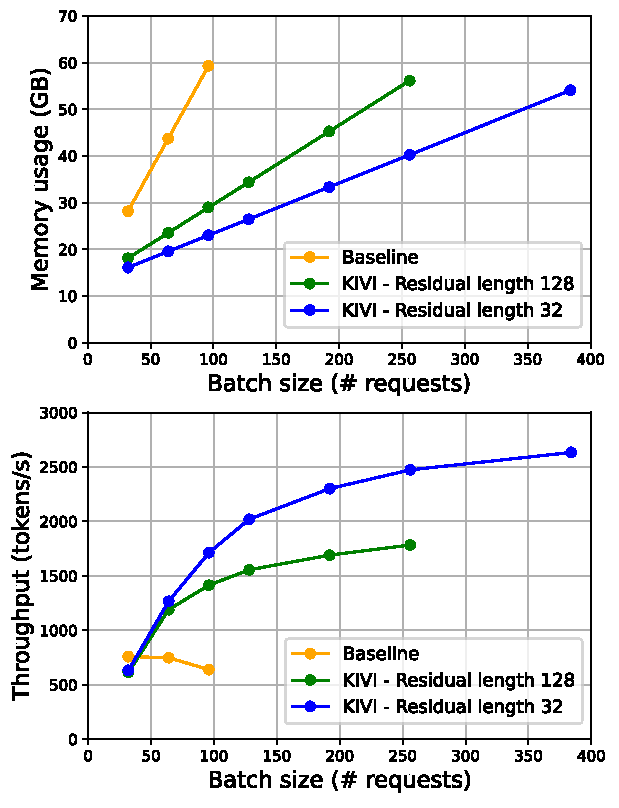
\includegraphics[width=0.39\textwidth]{figures/throughput.pdf}
  \end{center}
    \vspace{-1em}
  \caption{Memory usage and throughput comparison between 2bit \kivi{} and 16bit baseline. \kivi{} can achieve higher throughput by enabling a larger batch size.}
  \label{fig: throughput}
\end{figure}

\subsubsection{Efficiency Comparison}
\label{sec: efficiency}

To evaluate the wall-clock time efficiency of \kivi{},
following vLLM \citep{vllm}, we synthesize workloads based on ShareGPT \citep{shargpt}, which contain input and output
texts of real LLM services.
On average, the data set has an input prompt length $l_{\text{prompt}}$ of 161 and an output length $l_{\text{gen}}$ of 338 \citep{vllm}.
We increase the batch size until out of memory and report the peak memory usage and throughput between \kivi{} (with residual length 32 and 128) and FP16 baseline for the Llama-2-7B model.
The hardware here is a single NVIDIA A100 GPU (80GB).

As shown in Figure \ref{fig: throughput}, with similar maximum memory usage, \kivi{} enables up to $\mathbf{4\times}$ larger batch size and gives $\mathbf{2.35\times \sim 3.47\times}$ larger throughput.
This throughput number can grow larger with longer context length and output length.
We also note that \textbf{ this speed-up can be greatly increased if we further fuse the KV cache quantization process with previous operations.}
We leave it as one of future work.
% Besides the ShareGPT workload, we also report the memory and speed of \kivi with longer context and output length on synthesized workload.
